\chapter{Experiments and Results}
\label{experiments_and_results}


All experiments followed a similar general pattern of execution. 
This pattern of execution is described in detail in Section \ref{sec:experimental_setup}, which covers the general pipeline of the preparation, training and evaluation for each experiment.
Section \ref{sec:investigating_human_readable_channel} then describes the specific experiments and results of our investigations in to the human readable channel of code, whereas Section \ref{sec:investigating_the_computer_channel} covers the computer readable channel investivations.
The the results of the experiments combining these channels is presented in \ref{sec:investigating_combined_channels}, and further experiments into the dataset are presented in section \textbf{SECTION}


\section{Experimental Setup} % (fold)
\label{sec:experimental_setup}

\subsection{General Procedure} % (fold)
\label{sub:general_procedure}

% subsection general_procedure (end)

All our experiments were conducted in the same fashion, starting with a choice of dataset partition from Table \ref{table:thefinaldataset} that would be suitable to the investigation.
We would then tokenize the names and descriptions and other textual features, and if necessary extract the features we would from the code. 
These tokenization procedures and code extraction procedures are described in subsections \ref{sub:tokenizing_textual_input}, \ref{sub:tokenizing_argument_descriptions} and \ref{sub:tokenizing_code_features}.
After tokenization, the neural models would be trained on TESLA \textbf{GPUs}, for HOW long. 
These would evaluate performance on a dev set every epoch, and print translations.
How long did an epoch take.
When did we stop training.
Models were all evaluated by the same procedure as detailsed in section blah. 
%evaluated by assessing the BLEU, loss \& perplexity.


\subsection{Tokenizing Argument and Function Names} % (fold)
\label{sub:tokenizing_textual_input}

\subsection{Tokenizing Argument Descriptions} % (fold)
\label{sub:tokenizing_argument_descriptions}

\subsection{Tokenizing Code Features} % (fold)
\label{sub:tokenizing_code_features}

\subsection{Evaluation Procedure} % (fold)
\label{sub:evaluation_procedure}

% subsection evaluation_procedure (end)

% subsection tokenizing_code_features (end)

% subsubsection tokenizing_argument_descriptions (end)

% subsection tokenizing_textual_input (end)

% \subsubsection{Preparing the Data} % (fold)
% \label{ssub:Preparing the Data}

% \begin{enumerate}
%     \item All our data would come from one of the partitions of the dataset described in section \ref{sec:final_preparations}.

%     \item To tokenize variable names, function names and other arguments:
%     \begin{enumerate}
%         \item we generated a vocabulary of all possible tokens in valid python
%         \item We added separator tokens to the vocabulary, \mintinline{python}{"<SEPARATOR_1>"}
%         \item We then tokenizer as sequences of characters and adding an \mintinline{python}{"<END_OF_ARG>"} token to the end.
%     \end{enumerate}
    
%     \item To tokenize the argument descriptions:
%     \begin{enumerate}
%         \item We then generated a vocabulary for our training data by:
%         \begin{enumerate}
%             \item first generating a provisional vocabulary of tokens used more than 4 times in the training data.
%             \item if these words existed in our Glove embedding vocabulary they were added to our the final vocabulary. We used the  \mintinline{python}{glove.6B.200d.txt} file of 200d embeddings trained on 6 billion tokens for our Glove embeddings, (CITE). 
%             \item when this provisional list was exhausted we took the remaining most popular words, as defined by the Glove embedding file, to fill our final vocabulary to our designated "vocab-size"
%         \end{enumerate}
%         \item We then tokenized the descriptions by moving to lower case, removing new lines, and  tokenizing them using the nltk punkt tokenizer (\mintinline{python}{nltk.word_tokenize})
%         \item We then replaced out of vocabulary tokens with an \mintinline{python}{"<UNK>"} token, and finally bookending our descriptions with \mintinline{python}{"<START>"} and \mintinline{python}{"<END>"} tokens.
%         \item Path - seq?

%     \end{enumerate}



%     \item In cases of tokenized code: 
%      \begin{enumerate}
%          \item  In the case of tokenizing code paths, we first extracted the syntax tree from the source code, and traversed it exploring all paths between two nodes.
%          \item CONTINUE
%      \end{enumerate}

% \end{enumerate}

% Once these tokenizations were complete we were ready to train our models.

% \subsubsection{Training} % (fold)
% \label{ssub:training}


%     Our models were trained in the standard way:
%     \begin{enumerate}
%         \item The Rote Learner was trained determininstically, in this case using `ngram overlap' feature, as mentioned in\ref{sec:rote_learner_model}. It was evaluated with different random seeds 50 times on the hold out dataset.
%         \item The Seq-to-Seq model was trained using the backpropagation algorithm and adaptive momentum optimisation. The hyperparameters are presented in table X. 80 Epochs were evaluated, and the best and average scores were taken \textbf{EDIT}
%     \end{enumerate}




% \subsubsection{Evaluation} % (fold)
% \label{ssub:evaluation}

% % subsection training (end
% \begin{enumerate}



%     \item Finally when it came to evaluating our models on held-out datasets, we would ran translations on the dataset and calculated the BLEU score using the BLEU method found in \textbf{HERE}.
%     In particular BLEU scores were calculated over the whole corpus and \textbf{WHAT SMOOTHING HYPERPARAMTERS}.
%     \item It should be stressed that if a hyperparameter had to be tuned, it was always done on the validation set, with the test set untouched, until final evaluation. In the case of all neural models, the results presented are using the best hyperparameters under the validation set.

% \end{enumerate}

% section experimental_setup (end)

\section{Investigating Human Readable Channel} % (fold)
\label{sec:investigating_human_readable_channel}

% INVESTIGATION PURELY BASED ON NAME
\subsection{Comparing Baseline Models} % (fold)
\label{sub:comparing_baseline_models}

\subsubsection{Experiment Objective} % (fold)

As a baseline, we first wanted to investigate the informative power of simply the names of variables, with regards to different architectures of our baseline model.
We expected a reasonable signal to come from just the variable name which should be learnable by both our seq-to-seq model and rote learner. 

\subsubsection{Method \& Results} % (fold)

Since this experiment would only use the variable name to predict the descrption, we used the Reduced Random-Split Dataset listed in section.
This prevented inflation of BLEU scores due to exact matches being both in the train and validation set.

We then ran the standard tokenizations of input name on the Rote Learner, which only used the N-character-gram overlap criterion.
This was repeated 50 times, to provide an robust estimate of the standard deviation and mean BLEU scores, due to the inherent stocasticity to the model.

Then we ran a series of experiments on the basic Char-to-Seq architectures, starting from a basic seq-to-seq, then adding attention, a bidirectional encoder and finally dropout.
These best models were taken on the best BLEU scores up to 150 epochs, of training, and evaluated on the test and development set. % WHY 150

We report the BLEU scores in Table \ref{table:name_baseline} showing a strong performance from the Rote Learner of corpus level BLEU $9.03 \pm 0.32$ on validation and $10.60 \pm  0.30$. 
The Seq-to-Seq architectures initially underperformed the Rote Learner, scoring $7.76 $ and $  7.63$ on the validation and test set. However a marked improvement was seen by adding attention, as was adding the bidirectional encoder and dropout. 
The final model, with all addition beat the Rote Learner reasonably with a BLEU score of $12.46 $ and $12.72$ on validation and test set respectively.

The hyperparameters for these models are found in the Appendix, Table \ref{table:hyperparams_name_baseline}.
% ALL STOPPED at 150 EPOCHS. No improvement on best for 20 epochs, except original 146


\begin{table}[!ht]
\begin{center}
\begin{tabular}{ c | c | c }
    Model                             & BLEU (Validation)  & BLEU (Test)    \\
    \hline
    Rote Learner (x50)                & $ 9.03 \pm  0.32 $ & $ 10.60 \pm 0.27 $   \\
    \hline
    Seq to Seq                        & $ 8.97 $ & $ 8.18 $ \\
    + \textit{attention}              & $ 10.05 $ & $ 9.89 $  \\
    + \textit{bidirectional encoder}  & $ 11.76 $ & $ 12.34 $  \\
    + \textit{dropout}                & $ 12.68 $ & $ 12.72 $  \\
    \hline

    % Model                             & BLEU (Validation)  & BLEU (Test)    \\
    % \hline
    % Rote Learner (x50)                & $ 9.03242 \pm  0.31980 $ & $ 10.59658 \pm 0.26939 $   \\
    % \hline
    % Seq to Seq                        & $ 8.98624 $ & $ 8.17635 $ \\
    % + \textit{attention}              & $ 10.05134 $ & $ 9.88608 $  \\
    % + \textit{bidirectional encoder}  & $ 11.75615 $ & $ 12.34480 $  \\
    % + \textit{dropout}                & $ 12.67504 $ & $ 12.72236 $  \\
    % \hline
    % Seq to Seq                        & $ 4.60169 $ & $ 4.97880 $  \\
    % + \textit{attention}              & $ 4.81255 $ & $ 5.42022 $  \\
    % + \textit{bidirectional encoder}  & $ 3.00068 $ & $ 3.05952 $  \\
    % + \textit{dropout}                & $ 6.37864 $ & $ 6.33307 $  \\
    % \hline
\end{tabular}
\caption {Results of Experiment \ref{sub:comparing_baseline_models}: Comparing Baseline Models }
\label{table:name_baseline}
\end{center}
\end{table}



\subsubsection{Analysis} % (fold)

Most surprising of this result is the strength of the Rote Learner, despite there being no `exact matches' in the training and development sets. 
This is largely the result of there are arguments in the corpus with very similar descriptions, which may vary by only a few words. 

To investigate this we examined the predictions from the Rote Learner on the validation set. 
We evaluated the sentence level BLEU score on these, and found that although the vast majority evaluate to zero, a number of examples have a coincidental overlap in descriptions, resulting in a non negligible BLEU score. 
A random sample of these non-zero scored translations are presented in Figure \ref{tab:rotelearner_nameonly}.

With regard to the Seq-to-Seq, it is not surprising these standard additions to the seq-to-seq architecture improve the model. 
The addition of a bidirectional model adds capacity to the model by increasing the size of the hidden vector, and attention allows the model to condition sentence generation on the input, further adding complexity to the model.
The dropout also adds a regularizing effect.

It is perhaps surprising that the vanilla Seq-to-Seq struggles to outperform the Rote Learner. 
It is possible that the lack of contextualising information from attention results in an inability to learn from long description sequences that the Rote Learner can regurgitate immediately. 

However, once the attention and capacity are increased the results are explanatory.
The model synthesises similar (or even the same!) sequences of characters with their different descriptions, into a single description, which may fit better than randomly guessing from a bag of seen sequences. 

For instance, the most frequent argument, \mintinline[]{yaml}{name}, occurs in the train set 318 times with different descriptions. 
It also occurs 52 times in the validation set, again, with different descriptions. 
For each of these point the Rote Learner predicts a different description from the train set, on average scoring $0.00646 \pm 0.006$, whereas the Seq-to-Seq makes the same prediction each time, and scores $0.4029$, almost two orders of magnitude better, with the sensible average: ``name of the variable to return." 

In these cases the Seq-to-Seq model is interpolating in an overdetermined problem, and this highlights one of the advantages of neural networks in machine translation problems. 




\begin{table}
\begin{center}
\makebox[\linewidth][c]{
\begin{tabular}{l}
\hline\\

\textbf{A Random Sample of Bleu Scores $>0$ from Rote Learner on Random Split }\\\\ 


\textbf{Bleu Score}: 0.364
\textbf{Confidence}: 100.0\%  \\
\textbf{Argument}: \mintinline[]{python}{e d g e _ m a t c h}\\
\textbf{Description}: a function that returns true if the edge attribute dictionary for \\
the pair of nodes ( u1 , v1 ) in g1 and ( u2 , v2 ) in g2 should be considered equal during\\
the isomorphism test . if edge\_match is not specified then edge attributes are not considered .\\
\textbf{Prediction}: a function that returns true if the edge attribute dictionaries for\\
the pair of nodes ( $<$UNK$>$ , $<$UNK$>$ ) in $<$UNK$>$ and ( u2 , $<$UNK$>$ ) in $<$UNK$>$\\
should be considered equal during matching .\\

\\
\textbf{B}: 0.075
\textbf{C}: 11.1\%  \\
\textbf{A}: \mintinline[]{python}{u s e _ l o c k i n g}\\
\textbf{D}: ` bool ` . if true use locks for update operation .\\
\textbf{P}: an optional ` bool ` . defaults to ` true ` . an optional bool . defaults to\\
true . if true , the assignment will be protected by a lock ; otherwise the behavior is\\
undefined , but may exhibit less contention .\\
\\
\textbf{B}: 0.558
\textbf{C}: 12.5\%  \\
\textbf{A}: \mintinline[]{python}{y _ t r u e}\\
\textbf{D}: ground truth ( correct ) target values .\\
\textbf{P}: ground truth ( correct ) labels .\\
\\
\hline
\\
\end{tabular}
}
\end{center}
\caption{This is a random sample of sentence level BLEU scores that are non-zero fon the validation set for a Rote Learner}
\label{tab:rotelearner_nameonly}
\end{table}


% INVESTIGATION DIFFERENT TOKENIZATIONS
\subsection{Investigating Different Tokenizations} % (fold)
\label{sub:investigating_different_tokenizations}

\subsubsection{Experiment Objective} % (fold)

Having established a naive baseline and the validity of our neural approaches, we decided to investigate how other human names could help our translation problem.
We hypothesised that the names in the function signature could play an important role in contextualising an overdetermined or underdetermined variable name, further improving the performance of the LSTM relative to the Rote Learner.

\subsubsection{Method \& Results} % (fold)

We investigated how four different arrangements of input data would affect translation behaviour. 
These were:
just the argument name; the argument name with the function name; the argument name with co-argument names; and the argument name with both function name and co-argument names.

Once again we used the Reduced Random-Split Dataset, to prevent advantages due to duplicates, and ran the standard tokenization procedures outline in Sections X. 

As in section \ref{sub:comparing_baseline_models}, we ran 50 repetitions of the Rote Learner on these new tokenizations, to overcome the stochasiticity in their evaluations, once again using N-character-gram overlap as the matching criterion.

Then we ran four models of the Seq-to-Seq architectures, with attention, dropout and bidirectional encoders - just as the final model of section \ref{sub:comparing_baseline_models}. These ran for a maximum of 150 epochs, and the model with best BLEU score was selected. 

We report the results in Table \ref{table:tokenization}. 
In particular we note that in all cases the Rote Learner's performance improved with added information, in the best case, over three points to $12.22 \pm 0.23$ on validation and $14.34 \pm 0.21$ on test, thanks to the addition of the function name. 

The Seq-to-Seq model on the other hand benefitted less than the Rote Learner, if at all. In both tokenizations using other arguments, the model improved by approximately one point. However the tokenization involving the addition of just function name, saw a performance reduction of about 1.5 points, across both validation and test.

Although this agreed with out hypothesis that there is value in extra naming of variables, the under performance of the Seq-to-Seq model was surprising and is examined more fully in the analysis section.


The hyperparameters of these models are presented in Appendix Table \ref{table:hyperparams_different_tokenizations}


\begin{table}[!ht]
\begin{center}
\begin{tabular}{ c | c | c }
    Model                               & BLEU Validation            & BLEU Test  \\
    \hline
    \hline
    Rote Learner                        &                  & \\    
    - \textit{name only}                & $ 9.03  \pm  0.32 $ & $ 10.60 \pm 0.27 $  \\
    - \textit{name + function name}     & $ 12.23 \pm  0.23 $ & $ 14.34 \pm 0.22 $  \\
    - \textit{name + co-argument names}        & $ 12.06 \pm  0.16 $ & $ 14.22 \pm 0.16 $  \\
    - \textit{name + function name + co-argument names}  & $ 11.36 \pm  0.14 $ & $ 13.51 \pm 0.13 $ \\
    \hline
    \hline
    Seq to Seq                          &                  & \\
    - \textit{name only}                & $ 12.46441 $ & $ 12.72522 $  \\
    - \textit{name + function name}     & $ 10.77699 $ & $ 11.24894 $ \\
    - \textit{name + co-argument names}      & $ 13.69964 $ & $ 13.73890 $  \\
    - \textit{name + function name + co-argument names} & $ 14.13267 $ & $ 13.63351 $ \\
    % Model                               & BLEU Validation            & BLEU Test  \\
    % \hline
    % \hline
    % Rote Learner                        &                  & \\    
    % - \textit{name only}                & $ 9.03242  \pm  0.31980 $ & $ 10.59658 \pm 0.26939 $  \\
    % - \textit{name + function name}     & $ 12.22728 \pm  0.23408 $ & $ 14.33850 \pm 0.21622 $  \\
    % - \textit{name + co-argument names}        & $ 12.06262 \pm  0.16356 $ & $ 14.21676 \pm 0.16067 $  \\
    % - \textit{name + function name + co-argument names}  & $ 11.35728 \pm  0.13663 $ & $ 13.50626 \pm 0.13192 $ \\
    % \hline
    % \hline
    % Seq to Seq                          &                  & \\
    % - \textit{name only}    !!            & $ 12.46441 $ & $ 12.72522 $  \\
    % - \textit{name + function name} !!    & $ 10.77699 $ & $ 11.24894 $ \\
    % - \textit{name + co-argument names}  !!    & $ 13.69964 $ & $ 13.73890 $  \\
    % - \textit{name + function name + co-argument names}   !! & $ 14.13267 $ & $ 13.63351 $ \\
    % \hdashline
    % Seq to Seq                          &                  & \\
    % - \textit{name only}                & $ 5.54103 $ & $ 5.43827 $  \\
    % - \textit{name + function name}     & $ 4.76165 $ & $ 4.40557 $  \\
    % - \textit{name + other args}        & $ 5.70546 $ & $ 6.04723 $  \\
    % - \textit{name + function name + other args}     & $ 6.26783 $ & $ 6.24153 $ \\
    
    \hline
\end{tabular}
\caption {Investigate the effect of different code features}
\label{table:tokenization}
\end{center}
\end{table}


\subsubsection{Analysis} % (fold)
\label{ssub:analysis}

In order to probe the Seq-to-Seq model, we first investigated some of the typical setences generated by the model on the validation set.
We found that in general a number of different failings fell into either categories of overfitting or nonsense. 
Some typical examples of the model on the \textit{name + co-argument name} model are presented in Table \ref{table:typicalvarotherargs}, along with an example of a `plausible' translation. 


\begin{table}[ht!]
\begin{center}
\begin{tabular}{ l  }


\textbf{Overfitting}\\

\textbf{Input}: \mintinline[]{python}{e n c o d i n g _ t y p e <SEP-1> s e l f <SEP-2> d o c u m e}...\\
...\mintinline[]{python}{n t <SEP-2> r e t r y <SEP-2> t i m e o u t <SEP-2> <END>}\\
\textbf{Description}: the encoding type used by the api to calculate offsets .\\
\textbf{Prediction}: the encoding type used by the api to calculate sentence offsets . \\
\\\hline\\

\textbf{Nonsense}\\

\textbf{I}: \mintinline[]{python}{i n p u t <SEP-1> n a m e <SEP-2> <END>}\\
\textbf{D}: a ` tensor ` of type ` complex64 ` . a complex64 tensor .\\
\textbf{P}: ` $<$UNK$>$ ` , ` $<$UNK$>$ ` . shape is ` [ ... , m , m ] ` . \\
\\\hline\\

\textbf{Plausible}\\

\textbf{I}: \mintinline[]{python}{i n p u t <SEP-1> s t r u c t u r e <SEP-2> m a s k <SEP-2> o u t p}...\\
...\mintinline[]{python}{u t <SEP-2> b o r d e r _ v a l u e <SEP-2> o r i g i n <SEP-2> <END>}\\
\textbf{D}: binary image to be propagated inside ` mask ` .\\
\textbf{P}: binary image where a element is provided and a structuring element .\\
\\\hline\\

\\

\end{tabular}
\caption{Three examples of typical errors in the character Seq-to-Seq model.  In this case, the first example shows good use of data in the sequence but is nonsensical. The second is an example of overfitting where the predicted sentence is found in the dataset. The final case, multiple sequences such as these are found in the dataset, each with a different discription. Without looking at code, or function name (in this case) it is impossible to disambiguate and the model fails to make sense }
\label{table:typicalvarotherargs}
\end{center}
\end{table}

We then  visualized a number of attentions of the translations on the validation set, to investigate what the model was focusing on in these cases.
We found that, rather than being dispersed across multiple character tokens that might indicate useful phrases in the model, the attention focused overwhelmingly on the final tokens in the RNN in the vast majority of cases.
The attentions of the `plausible' and `nonsense' examples from  Table \ref{table:typicalvarotherargs} are visible in Figure ~\ref{fig:otherarg_attn}, demonstrating this.

\begin{figure}[ht!]
\begin{center}
    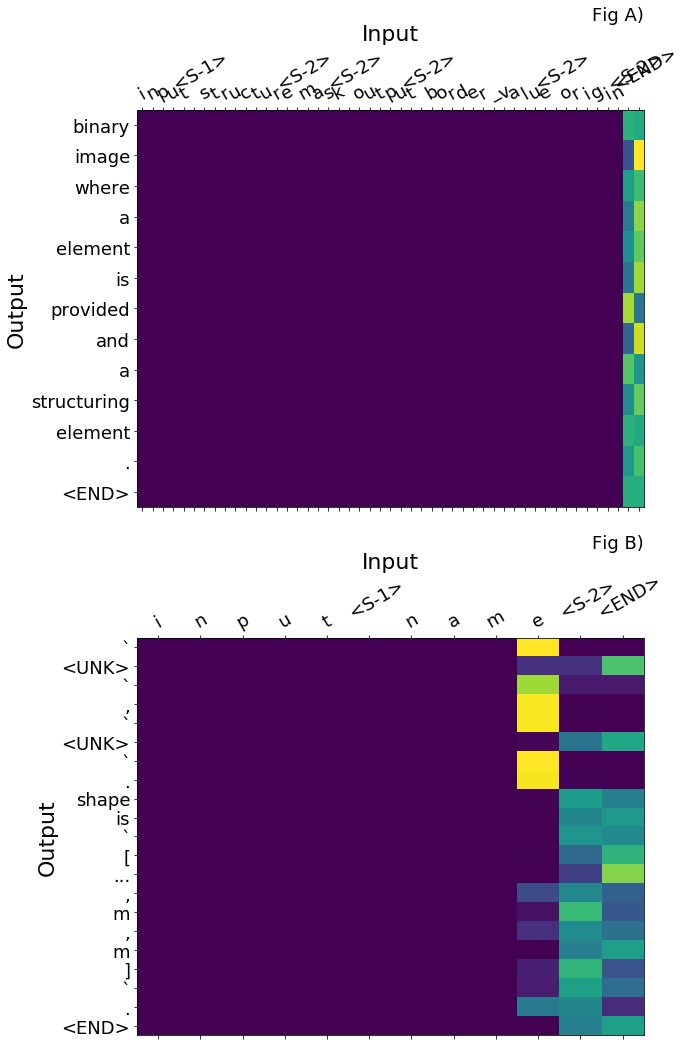
\includegraphics[width=0.7\linewidth]{images/otherargs_example.png}
    \caption{An example of some the attentions of from the Name + Other Arguments tokenization on a Seq-to-Seq model, on the Reduced Random-Split Dataset. Fig A) is a picture of a typical example, Fig B) bottom is an example that is very overdetermined.}
    \label{fig:otherarg_attn}
\end{center}
\end{figure}

This implies the model is using all the extra information to encode a single vector to contextualise on, rather than learning to apply parts of the sequence to parts of translation, in an alignment fashion.
This single contextual vector can contain all the sequence information because the encoded RNN outputs at N can contain information from the previous N-1 tokens, and this in principle allows the model the condition word generation on the all the information up to the `attended' input token. 

Although this behaviour was expected for short sequences like variable names, we expected longer sequences (of up to 120 tokens) to be harder to compress, and suspected overcapacity of the LSTM might allow this learning strategy to take place. 
With less capacity, perhaps the final output of the RNN would not be as informative, instead relying on outputs at different points of the sequence
However, repeating the experiment with an LSTM encoder size of 75 resulted in the same pattern of attention, though with a much reduced BLEU score.

We also repeated the experiment on the much larger Full Random-Split dataset, where now just the input argument name would be certainly be the most important feature, due to repetitions points with the same name with the same description, but different co-arguments and function names. 
In this case we saw the final heavy attention shift to the separator just after the variable name - indicating that the model was learning where the most informative section of the data was, but was still choosing the encoded vector at that point. 
Interestingly we found that model did still take into account the rest of the sequence after this point (generating different translations), but that these all varied along a the same theme of the variable name. 
The attentions for a single example are given in Figure ~\ref{fig:otherarg_attn_full_dataset}

\begin{figure}

\begin{center}
    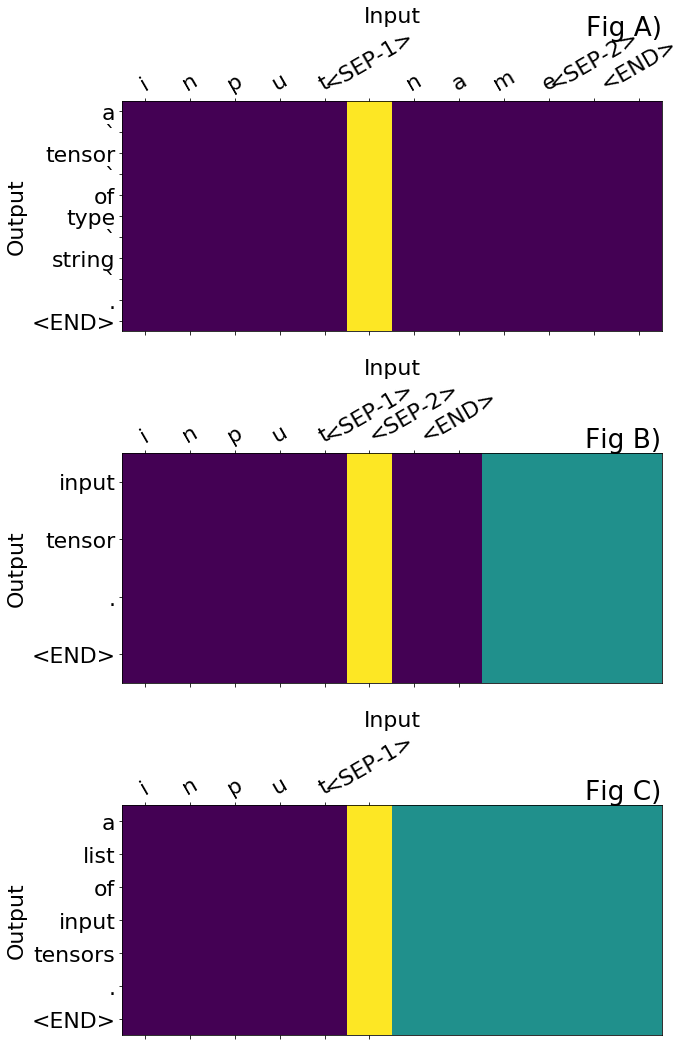
\includegraphics[width=0.7\linewidth]{images/different_translations_dupsXotherargs_3230minib.png}
    \caption{Three translations and attentions for an example of some the attentions of from the Name + Other Arguments on the tokenization on a Seq-to-Seq model trained on the Full Random-Split Dataset. Here is shows that, on the Full Random-Split Dataset, the most important feature is variable name, and the model attends solely to that, but that the hidden state of the LSTM still takes into account characters after the variable input }
    \label{fig:otherarg_attn_full_dataset}
\end{center}
\end{figure}

The conclusion to be drawn from this investigation is that the attention does not distribute well over characters, and these tokenizations actually behave much like longer single names, rather than features that can be distiguished separately. 
This leads to overfitting in many cases, as the some names are closer to unique, and you get a model that fits more like a Rote Learner. 
The model seems to work at its best when synthesising information as much as possible, but this seems more difficult to do when so much identifying information is given without information on redundancy. 
To give an example, Table \ref{table:example_plausible_training} shows the `plausible' example given above, with all training instances that start \mintinline[]{yaml}{input<SEP-1>structure}, highlighting that certain features of the final description are in the training ("binary image"), yet the potentially helpful sequence \mintinline[]{yaml}{<SEP-1>mask<SEP-1>} is ignored.

To counter this beahaviour in future, more work could be done both by investigating tokenizations or attention mechanisms.
In particular, the peaky nature of the softmax in attention could be replaced with a broader distribution, or the entropy of the softmax could be changed with a temperature parameter throughout training, to force the model to consider different sections of the data.
Ideally, combined with this differnet annention arrangement, more data would be provided that could help present a nuance to the arguments, rather than them simply being specifying information. 
Future work should at least investigate whether data augmentation by providing duplicates with arguments in different orders, perhaps also with synonyms of descriptions, could help models learn more generalisable descriptions.


\begin{table}
\begin{center}
\makebox[\linewidth][c]{
\begin{tabular}{l}

\hline
\textbf{Validation Example}\\

\textbf{I}: \mintinline[]{python}{i n p u t <SEP-1> s t r u c t u r e <SEP-2> m a s k <SEP-2> o u t p}...\\
...\mintinline[]{python}{u t <SEP-2> b o r d e r _ v a l u e <SEP-2> o r i g i n <SEP-2> <END>}\\
\textbf{D}: binary image to be propagated inside ` mask ` .\\
\textbf{P}: binary image where a element is provided and a structuring element . $<$END$>$\\
\\\hline\\

\textbf{Training Examples} starting \mintinline[]{yaml}{i n p u t <SEP-1> s t r u c t u r e}\\
\textbf{I}: \mintinline[]{yaml}{i n p u t <SEP-1> s t r u c t u r e 1 <SEP-2> s t r u c t u r}...\\
...\mintinline[]{yaml}{e 2 <SEP-2> o u t p u t <SEP-2> o r i g i n 1 <SEP-2> o r i g i n 2 <SEP-2> <END>}\\
\textbf{D}: binary image where a pattern is to be detected .\\
\\
\textbf{I}: \mintinline[]{yaml}{i n p u t <SEP-1> s t r u c t u r e <SEP-2> i t e r a t i o n s <SEP-2> o u t }...\\
...\mintinline[]{yaml}{p u t <SEP-2> o r i g i n <SEP-2> m a s k <SEP-2> b o r d e r _ v a l u e }\\
...\mintinline[]{yaml}{<SEP-2> b r u t e _ f o r c e <SEP-2> <END>}\\
\textbf{D}: binary array\_like to be closed . non-zero ( true ) elements form the subset to be closed .\\
\\
\textbf{I}: \mintinline[]{yaml}{i n p u t <SEP-1> s t r u c t u r e <SEP-2> o u t p u t <SEP-2> o r}...\\
...\mintinline[]{yaml}{i g i n <SEP-2> <END>}\\
\textbf{D}: n-dimensional binary array with holes to be filled\\
\\
\textbf{I}: \mintinline[]{yaml}{i n p u t <SEP-1> s t r u c t u r e <SEP-2> o u t p u t <SEP-2> <END>}\\
\textbf{D}: an array-like object to be labeled . any non-zero values in ` input ` are counted as features...\\
...and zero values are considered the background .\\
\\
\textbf{I}: \mintinline[]{yaml}{i n p u t <SEP-1> s t r u c t u r e <SEP-2> i t e r a t i o n s <SEP-2> m a s k }...\\
...\mintinline[]{yaml}{<SEP-2> o u t p u t <SEP-2> b o r d e r _ v a l u e <SEP-2> o r i g i n <SEP-2>}\\
...\mintinline[]{yaml}{b r u t e _ f o r c e <SEP-2> <END>}\\
\textbf{D}: binary image to be eroded . non-zero ( true ) elements form the subset to be eroded .\\
\\
\textbf{I}: \mintinline[]{yaml}{i n p u t <SEP-1> s t r u c t u r e <SEP-2> i t e r a t i o n s <SEP-2> m a s k}...\\
...\mintinline[]{yaml}{<SEP-2> o u t p u t <SEP-2> b o r d e r _ v a l u e <SEP-2> o r i g i n <SEP-2>}\\
...\mintinline[]{yaml}{b r u t e _ f o r c e <SEP-2> <END>}\\
\textbf{D}: binary array\_like to be dilated . non-zero ( true ) elements form the subset to be dilated .\\
\\



\end{tabular}
}
\caption{A validation example and the a selection of training points. Despite being a long sequence, }
\label{table:example_plausible_training}
\end{center}
\end{table}

%%% EXTRA PLOTS: Avergae attention over words
%%%.             Attention/Results of words shuffled



% What is the problem? Attention softmax is narrow and doesnt distribute well over characters, since there isn't really a one to one alignment. Instead what we see is the same behaviour as a much longer function name, where it works best when interpolating data. then give the plausibility

% Future work: Attention softmax is too narrow. Try a higher entropy distribution for character model
% Try a learning schedule
% Rotate the order of words, (done)
% Also more data.


% \begin{enumerate}
%     % \item we expected words to help choose bits in overdetermined cases. attention distributed across multiple words
%     % \item however we get attention focused on last word.
%     % \item The rnn final state acts as a good contextual vector for generation, we get good performance improvements on decoding
%     % \item The sort bonus is explained, but no change with longer.
%     \item It is possible the attention is being pathological. It's such a good strategy, that it stays there, and stops looking elsewhere, the weight decays to zero
%     % \item To investigate we ran with low lstm, -> no change in behaviour (LSTM 75), still tries to encode
%     \item We then tried to investigate if the rest of the data is being used (use the full dataset, and found that)
%     \item in cases with still degeneracy, attention is confused it panics (see bluring at end - can only explore nearest by states)
%     \item Check out Rote learner vs LSTM for "name" again. is it interpolating, or being a bad lstm (fitting bits of it, that dont transfer.)
%     \item We also take a closer look at the failures and notice a specific pattern. note tha in some cases the model works well, and. Basically hypothesise the size of the data with lack of indentifyin ginformation leads to overfitting, rather than just variable name which works.
% \end{enumerate}


\section{Investigating the Computer Readable Channel} % (fold)
\label{sec:investigating_the_computer_channel}

\subsection{Comparing Code2Vec to Baselines} % (fold)
\label{sub:comparing_code2vec_to_baselines}


\subsubsection{Experiment Objective} % (fold)

In our first examination of the computer readable channel we aimbed to validate our initial hypothesis that simply the code could be informative when predicting argument descriptions.
In particular we wished to assess what possible tokenizations of code paths from the syntax tree could prove most informative, and set up as strong baseline as possible against which would compare our neural model.



\subsubsection{Method \& Results} % (fold)

For this experiment we used the Full Random-Split Dataset, to make the most of the different code paths associated with each argument.
We followed the vocabulary generation and source code tokenization procedures outlined in section X. 
We used a vocabulary size of 15000 for both path strings and terminal nodes, and set the maximum number of paths per argument to  5000.
These values were sought to be as large as possible for the size of the GPU. 

We then ran our Rote Learner, using the four different matching code path only criteria, outlined in section X. 
These chose a description from a set of training samples by:
    \begin{itemize}
        \item combining samples with largest subpath overlap for each path in test, and chosing from that list. (Sub Path Proportional)
        \item combining samples with largest subpath overlap for each path in test, and chosing from the most frequent training point(s) in that list. (Sub Path Max)
        \item combining samples full overlap for each path in test, and chosing from that list (Full Path Proportional)
        \item combining samples full overlap for each path in test, and chosing from the most frequent training point(s) in that list. (Full Path Max)
    \end{itemize}
Each of these was run 50 timesto overcome the stochasticity of the Rote Learner.

We then ran the Code2Vec Decoder, following the usual training procedure, for a maximum of 100 epochs.
We selected the model with the best BLEU score in that time.
The hyperparameters for this model are found in Table {X}.

We report our results in Table \ref{table:name_code2vec_solo}, noting that the Rote Learner performed best using the Full Path Max matching, with a BLEU score $ 11.82 \pm  0.16 $ and  $ 12.61 \pm 0.12 $ on validation and test, but that the Code2Vec Decoder significantly outperformed this, achieving a BLEU score of $ 18.94 $ and $ 18.13 $ on validation and test respectively.

From the Rote Learning perspective, the next best criterion was the Sub Path Max, which achieved a corpus level BLEU score of $ 6.93 \pm  0.34 $ and $ 7.09 \pm 0.22 $ on validation and test respectively.  
The two remaining Proportional criteria performed worst, each about 6 bleu points worse than their counterparts

These results confirmed that looking at code paths would indeed be informative, and indicated that investigating full codepaths would indeed be the best way to start. 
They also showed great promise for the Code2Vec Decoder as a model.

% subsection comparing_code2vec_to_baselines (end)

\begin{table}[ht!]
\begin{center}
\begin{tabular}{ c | c | c  }
    Model                             & BLEU Validation  & BLEU Test      \\
    \hline
    Rote Learner (codeonly)                  &  &  \\
    - \textit{Subpath Proportional}              & $ 0.71 \pm  0.13 $ & $ 0.74 \pm 0.07 $   \\
    - \textit{Subpath Max}                       & $ 6.93 \pm  0.34 $ & $ 7.09 \pm 0.22 $  \\
    - \textit{Full Path Proportional}            & $ 4.94 \pm  0.28 $ & $ 5.11 \pm 0.18 $  \\
    - \textit{Full Path Max}                     & $ 11.82 \pm  0.16 $ & $ 12.61 \pm 0.12 $  \\
    \hline
    Code2Vec Decoder                             & $ 18.94 $ & $ 18.13 $  \\
    % \hdashline
    % Code2Vec                          & $ 12.64199 $ & $ 12.80257 $  \\
    \hline 
    % Model                             & BLEU Validaion  & BLEU (Test)      \\
    % \hline
    % Rote Learner (codeonly)           &  & & \\
    % - \textit{softest}                     & $ 0.70702 \pm  0.13979 $ & $ 0.73623 \pm 0.07094 $   \\
    % - \textit{soft}                        & $ 6.93465 \pm  0.33987 $ & $ 7.09349 \pm 0.21836 $  \\
    % - \textit{hard}                        & $ 4.94109 \pm  0.28153 $ & $ 5.11432 \pm 0.18345 $  \\
    % - \textit{hardest}                     & $ 11.82453 \pm  0.15695 $ & $ 12.61319 \pm 0.12093 $  \\
    % \hline
    % Code2Vec   !!                            & $ 18.93630 $ & $ 18.12909 $  \\
    % % \hdashline
    % % Code2Vec                          & $ 12.64199 $ & $ 12.80257 $ & \\
    % \hline
\end{tabular}
\caption {BLEU Scores on the Full Random-Split Dataset, for Code2Vec Decoder and a series of code only Rote Learners}
\label{table:name_code2vec_solo}
\end{center}
\end{table}

\subsubsection{Analysis} % (fold)
\label{ssub:analysis}

In order to investigate the behaviour of the Code2Vec model, we sampled points from the validation set, printed out the source code, paths and attentions as they passed through the model.
We observed that sometimes the model overfit some particular paths, with very high attentions on a single point, but more often than not the model distributed its attention over 4 or 5 paths, even if there were thousands to choose from.

A single example of such an analysis, where multiple paths are attended and the different paths are easy to see, is presented in Figure  \ref{fig:single_examples} .
It shows the pretokenized syntax tree, the attented paths, the source and the translation.
From this example it is interesting to note that the model has chosen two paths that indicate list comprehensions feature in the variable, and it has inferred that a list should feature in the description from the code alone.

Noting that the model seemed to be performing as expected on a microscopic level, we continued to investigate the behaviour of the model across the entire validation set. 
Figure \ref{fig:entropy_code2vec} shows a the distribution of the entropies of the attentions of the Code2Vec vectors, for each point in the validation set. 
Presented along side, is the distribution of entropies that would have occured if every data point in the validation set had attained a uniform, categorical distribution as attention. 


Although this metric is prone to low scores on individual sentences <CITE> over the whole corpus, we can use it to get a sense for where the performance improvements come from.
These are presented in Figureand show both a significant increase in the models 1.0 scoring sentences, and also a modest increase in low scoring sentences. This indicates both an improvement that may be down to some form of overfitting (the model is able to find arguments that are very similar, and have similar code paths), but also an improvement due to generating just a few of the correct words, as in the example presented above. 


It is also interesting to note that the attention patterns observed in the example above also hold on a macroscopic scale. By taking the distribution of entropies of each of the attentions.




\begin{enumerate}
    \item With the code lstm we see some of the behaviour we like, but also, only overfitting. There is no sequence so in some cases, a path or a single variable can be informative, but it performs well.
    \item See a single example and distribution of attention.
    \item CLearly there are a lot of spikes compared to uniform. More masking the more spiking, though this is partly due to best bleu. Compare at cross entropy time?
    \item Then look at, bleu per sentence, maybe av bleu per sentence per attn entropy.
    \item Big COMPARE vs ROTE LEARNER - can we conclude this is worth more researcg?
    \item Cna show how choices change w model for given example??

    \item C2VEnc: does combining add anythin? More capacity, check weights.
\end{enumerate}

% \begin{table}
\begin{listing}[h!] 
\begin{center}

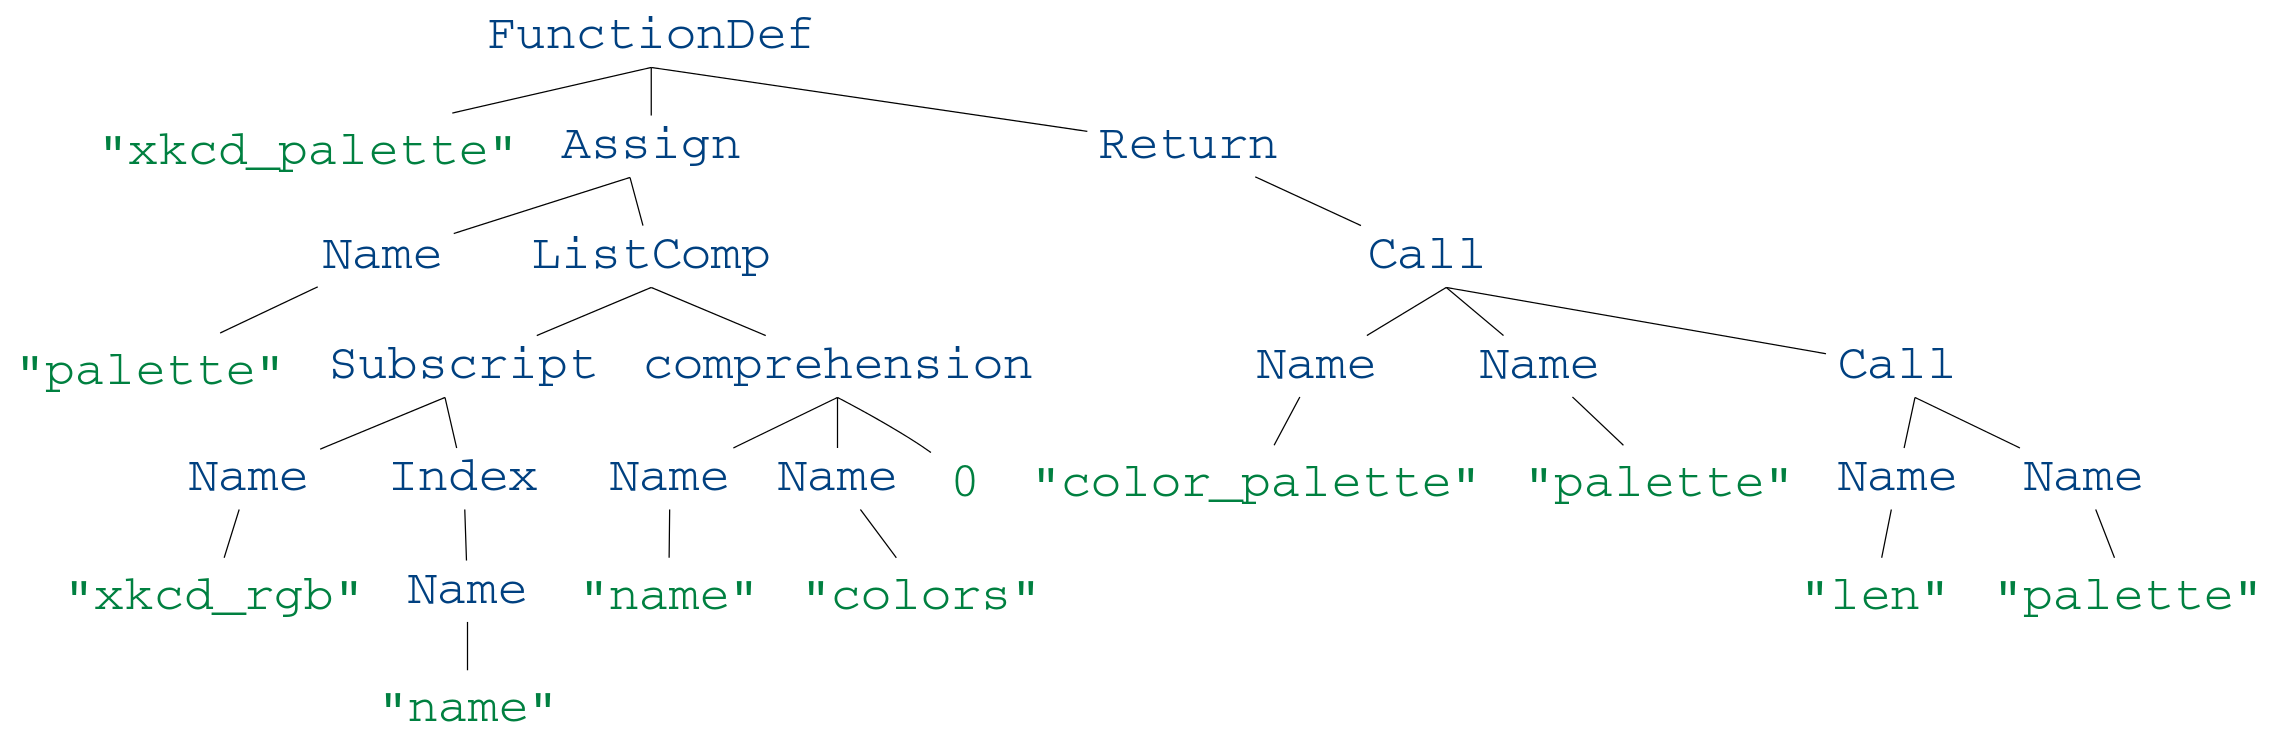
\includegraphics[width=\linewidth]{ImagesCodeRelated/xkcd_palette_strip.png}
\begin{minted}[]{python}
def xkcd_palette(colors):
    palette = [xkcd_rgb[name] for name in colors]
    return color_palette(palette, len(palette))

\end{minted}
\begin{tabular}{l}
\textbf{I}: \mintinline[]{python}{colors}\\
\textbf{D}: list of keys in the `` seaborn.xkcd\_rgb `` dictionary .\\
\textbf{P}: a list of data to read . if none , all other the first will be returned .\\
\end{tabular}


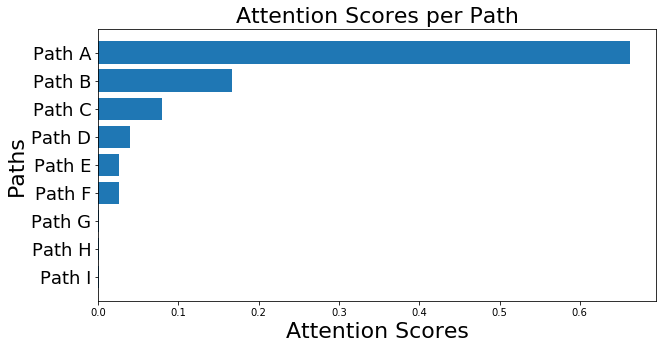
\includegraphics[width=0.8\linewidth]{ImagesCodeRelated/attention_xkcd.png}
        % how to set font size here to 10 px ?  
\begingroup
    \fontsize{10pt}{12pt}\selectfont
\begin{tabular}{c l}
    & \textbf{Paths} \\
    \\
    \textbf{Path A} & Name $\leftarrow$ comprehension $\leftarrow$ ListComp $\leftarrow$ Assign $\rightarrow$ Name : \mintinline[]{yaml}{palette} \\
    \textbf{Path B} & Name $\leftarrow$ comprehension $\leftarrow$ ListComp $\leftarrow$ Assign $\leftarrow$ FunctionDef[...] \\
        & [...]$\rightarrow$ Assign $\rightarrow$ ListComp $\rightarrow$ comprehension : \mintinline[]{yaml}{<UNK>} \\
    \textbf{Path C} & $<$UNK$>$ : \mintinline[]{yaml}{color_palette} \\
    \textbf{Path D} & Name $\leftarrow$ comprehension $\rightarrow$ Name : \mintinline[]{yaml}{name} \\
    \textbf{Path E} & $<$UNK$>$ : \mintinline[]{yaml}{palette} \\
    \textbf{Path F} & $<$UNK$>$ : \mintinline[]{yaml}{palette} \\
    \textbf{Path G} & $<$UNK$>$ : \mintinline[]{yaml}{len} \\
    \textbf{Path H} & $<$UNK$>$ : \mintinline[]{yaml}{name} \\
    \textbf{Path I} & $<$UNK$>$ : \mintinline[]{yaml}{<UNK>} \\
\end{tabular}
\endgroup

% \caption{Example Attention Scores}
% \end{table}

\end{center}
\caption{Code \& List}
\label{fig:single_examples}
\end{listing}



\begin{figure}
\begin{center}
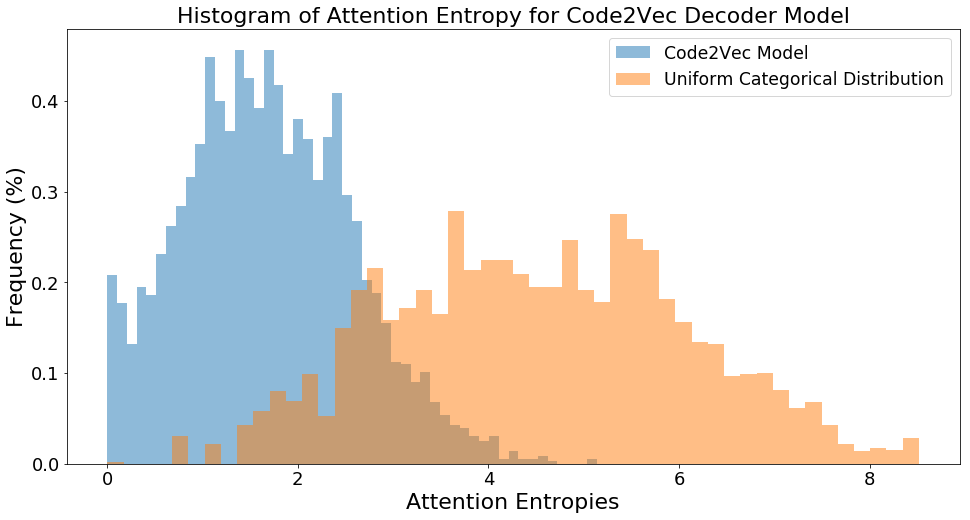
\includegraphics[width=0.8\linewidth]{ImagesCodeRelated/code2vec_entropies.png}
\end{center}
\label{fig:entropy_code2vec}
\end{figure}


% subsubsection analysis (end)





\subsection{Comparing Code2Vec Altered} % (fold)
\label{sub:comparing_code2vec_altered}

\subsubsection{Experiment Objective} % (fold)

The Code2Vec Decoder model uses a vocabulary of terminal nodes to generate code paths. 
Due to the python abstract syntax tree, these are almost always names, which could be either those of internal variables, built-in functions or even out of scope objects. 
We investigated masking these terminal node names, to be conclude that that the structure of the code was providing a valuable signal to the Code2Vec Decoder, beyond the ideosyncracies of variable and method naming.

\subsubsection{Method \& Results} % (fold)

By using the code2vec tokenization of paths outlined in section X, we extracted all paths for each argument in question from the AST of the code. 
The outputs of the result are presented in Table \ref{table:name_code2vec_solo}.

\subsubsection{Analysis} % (fold)

Checkout the weights now that the masking has taken place. Is it genuinely lerning good patters? What are good patterns? Whats an example of whats been classified and what being referred to in the syntax tree?


\begin{table}[ht!]
\begin{center}
\begin{tabular}{ c | c | c | c }
    Model                             & BLEU (Unsplit)  & BLEU (Split)    & Perpelexity \\
    \hline
    Rote Learner (best performer)          & $ 11.82453 \pm  0.15695 $ & $ 12.61319 \pm 0.12093 $ & \\
    \hline
    Code2Vec                !!              & $ 18.93630 $ & $ 18.12909 $ & \\
    Code2Vec (masked args)  !!              & $ 17.01868 $ & $ 16.93701 $ & \\                  
    Code2Vec (masked all)   !!               & $ 13.27677 $ & $ 13.07374 $ & \\
    % \hdashline

    % Code2Vec                              & $ 12.64199 $ & $ 12.80257 $ & \\
    % Code2Vec (masked args)                & $ 12.10462 $ & $ 11.93314 $ & \\
    % Code2Vec (masked all)                 & $ 9.01463 $ & $ 9.15697 $ & \\
    \hline
\end{tabular}
\caption {Investigate code2vec but with masked variables}
\label{table:code_2_vec_masked}
\end{center}
\end{table}


\begin{figure}
\begin{center}
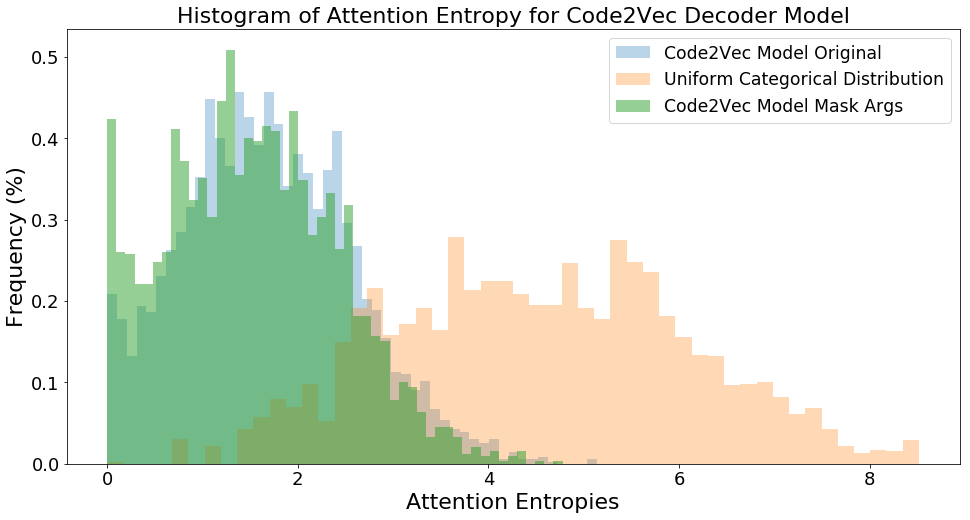
\includegraphics[width=0.8\linewidth]{ImagesCodeRelated/entropies_mask_args.png} 
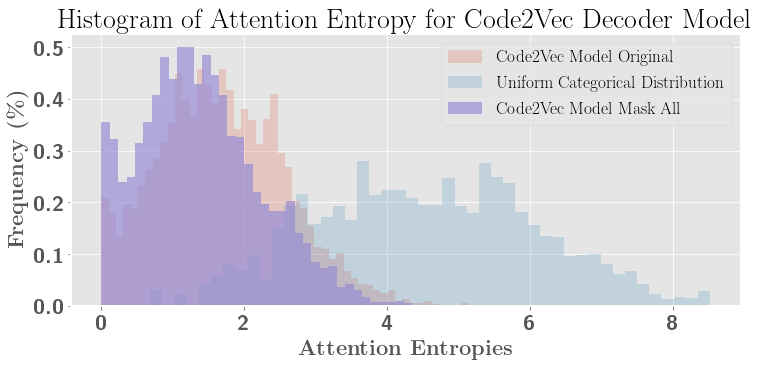
\includegraphics[width=0.8\linewidth]{ImagesCodeRelated/entropies_mask_all.png}
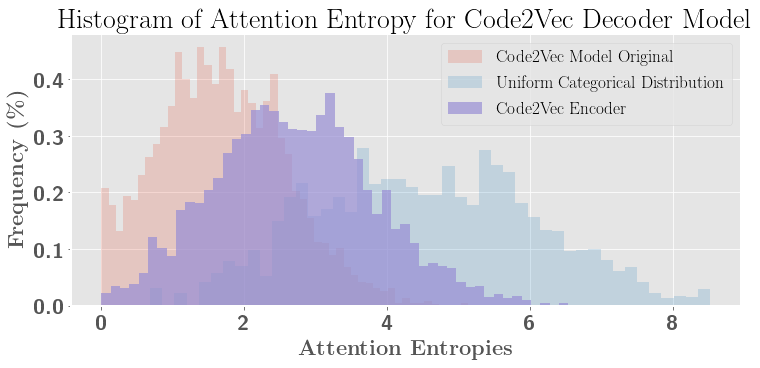
\includegraphics[width=0.8\linewidth]{ImagesCodeRelated/entropies_encoder.png}
\end{center}
\end{figure}



\begin{figure}
\begin{center}
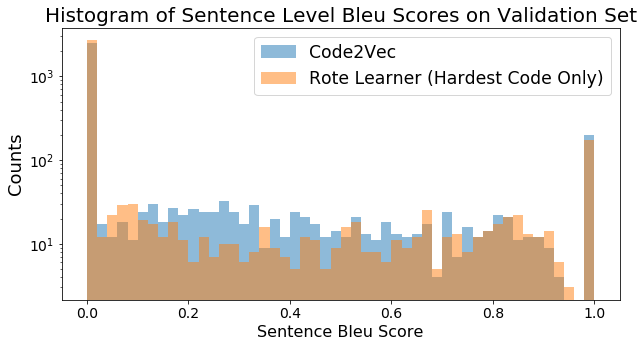
\includegraphics[width=0.8\linewidth]{ImagesCodeRelated/SentenceBleuCodeonly.png}
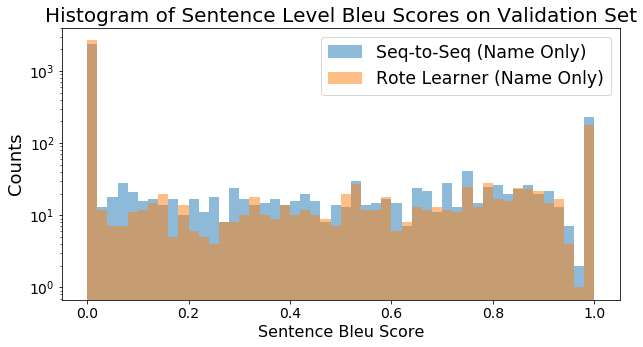
\includegraphics[width=.8\linewidth]{ImagesCodeRelated/SentenceBleuNameOnly.png}
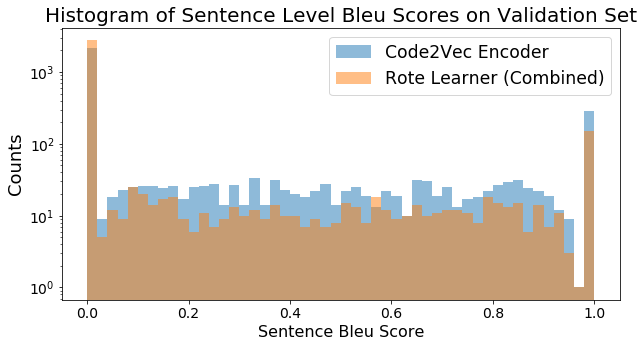
\includegraphics[width=.8\linewidth]{ImagesCodeRelated/SentBleuCombined.png}
\end{center}
\end{figure}






\section{Investigating Combined Channels} % (fold)
\label{sec:investigating_combined_channels}


\subsection{Combined Code2Vec } % (fold)
\label{sub:combined_code2vec}

% subsection comparing_code2vec_to_baselines (end)

\begin{table}[h!]
\begin{center}
\begin{tabular}{ c | c | c | c }
    Model                             & BLEU (Unsplit)  & BLEU (Split)    & Perpelexity \\
    \hline
    Rote Learner  (code only)        & $ 11.83875 \pm  0.15697 $ & $ 12.62479 \pm 0.12103 $ & \\
    Code2Vec  (code only)         !!    & $ 18.93630 $ & $ 18.12909 $ & \\
    % \hdashline
    % Code2Vec  (code only)             & $ 12.64199 $ & $ 12.80257 $ & \\
    \hline
    \hline
    Rote Learner  (name only)         & $ 19.03534 \pm  0.35183 $ & $ 19.68826 \pm 0.28100 $ & \\
    Seq2Seq  (name only)      !!         & $ 26.39189 $ & $ 25.39841 $ & \\
    % \hdashline
    % Seq2Seq  (name only)              & $ 15.94701 $ & $ 15.71091 $ & \\
    \hline
    \hline
    Rote Learner (combined)            & $ 15.01764 \pm  0.44897 $ & $ 15.75528 \pm 0.29560 $ & \\
    Code2Vec  + Char to Seq       !!     & $ 28.76581 $ & $ 27.68100 $ & \\
    % \hdashline
    % Code2Vec  + Char to Seq           & $ 23.11775 $ & $ 22.37520 $ & \\
    \hline
\end{tabular}
\caption {Investigate code2vec combined with seq to seq}
\label{table:code2vec_embed}
\end{center}
\end{table}

\subsubsection{Experiment Objective} % (fold)

\begin{itemize}
    \item finally we decide to combine
    \item we dont see a great improvemet separately, how about together?
    \item surprised
\end{itemize}


\subsubsection{Method \& Results} % (

\subsubsection{Analysis} % (fold)

Attentio here will be important. 
How do the code2vec vectors change direction when using names as well as code!
Weights etc

\section{Analysis} % (fold)
\label{sec:analysis}

% section sundry_analysis (end)

\subsection{Investigating the Removal of Duplicates} % (fold)
\label{sub:investigating_the_removal_of_duplicates}

\subsubsection{Experiment Objective} % (fold)

We now want to check whether generalisation is possible across results. 
We take the best models and repeat them on th esplit dataset.

\subsubsection{Method \& Results} % (


\begin{table}[!ht]
\begin{center}
\begin{tabular}{ c | c | c | c }
    Model                             & BLEU (Unsplit)  & BLEU (Split)    & Perpelexity \\
    \hline
    Rote Learner  (code only)         & $ 1.01257 \pm  0.11410 $ & $ 0.84707 \pm 0.04996 $ & \\
    Code2Vec                     !!   & $ 0.88741 $ & $ 0.89466 $ & \\
    Code2Vec  (mask args)             & $ 0.66894 $ & $ 0.67366 $ & \\
    Code2Vec  (mask alls)             & $ 0.69457 $ & $ 0.71360 $ & \\
    \hline
    \hline
    Rote Learner  (name only)         & $ 1.43480 \pm  0.16744 $ & $ 1.36063 \pm 0.06452 $ & \\
    \hline
    Seq2Seq                             & &  & \\
    - \textit{name only}              & $ 1.53474 $ & $ 1.58206 $ & \\
    - \textit{name + function name}      & $ 1.54843 $ & $ 1.52191 $ & \\
    - \textit{name + other args}         & $ 1.53296 $ & $ 1.45225 $ & \\   
    - \textit{name + function name + other args}     & $ 1.50983 $ & $ 1.48267 $ & \\
    \hline
    \hline
    Rote Learner (combined)            & $ 1.23201 \pm  0.16873 $ & $ 1.15672 \pm 0.10083 $ & \\
    Code2Vec  + Char to Seq        !!      & $ 1.84887 $ & $ 1.58697 $ & \\\\
    \hline
\end{tabular}
\caption {Investigate split datasets}
\label{table:split_datasets_embed}
\end{center}
\end{table}


\subsection{Visualising Attention Weights} % (fold)
\label{sub:visualising_attention_weights}

